\section{Methodology}

Figure~\ref{fig:architecture} presents our system architecture, showing the complete pipeline from data ingestion through LLM regime detection.

\begin{figure*}[!htbp]
\centering
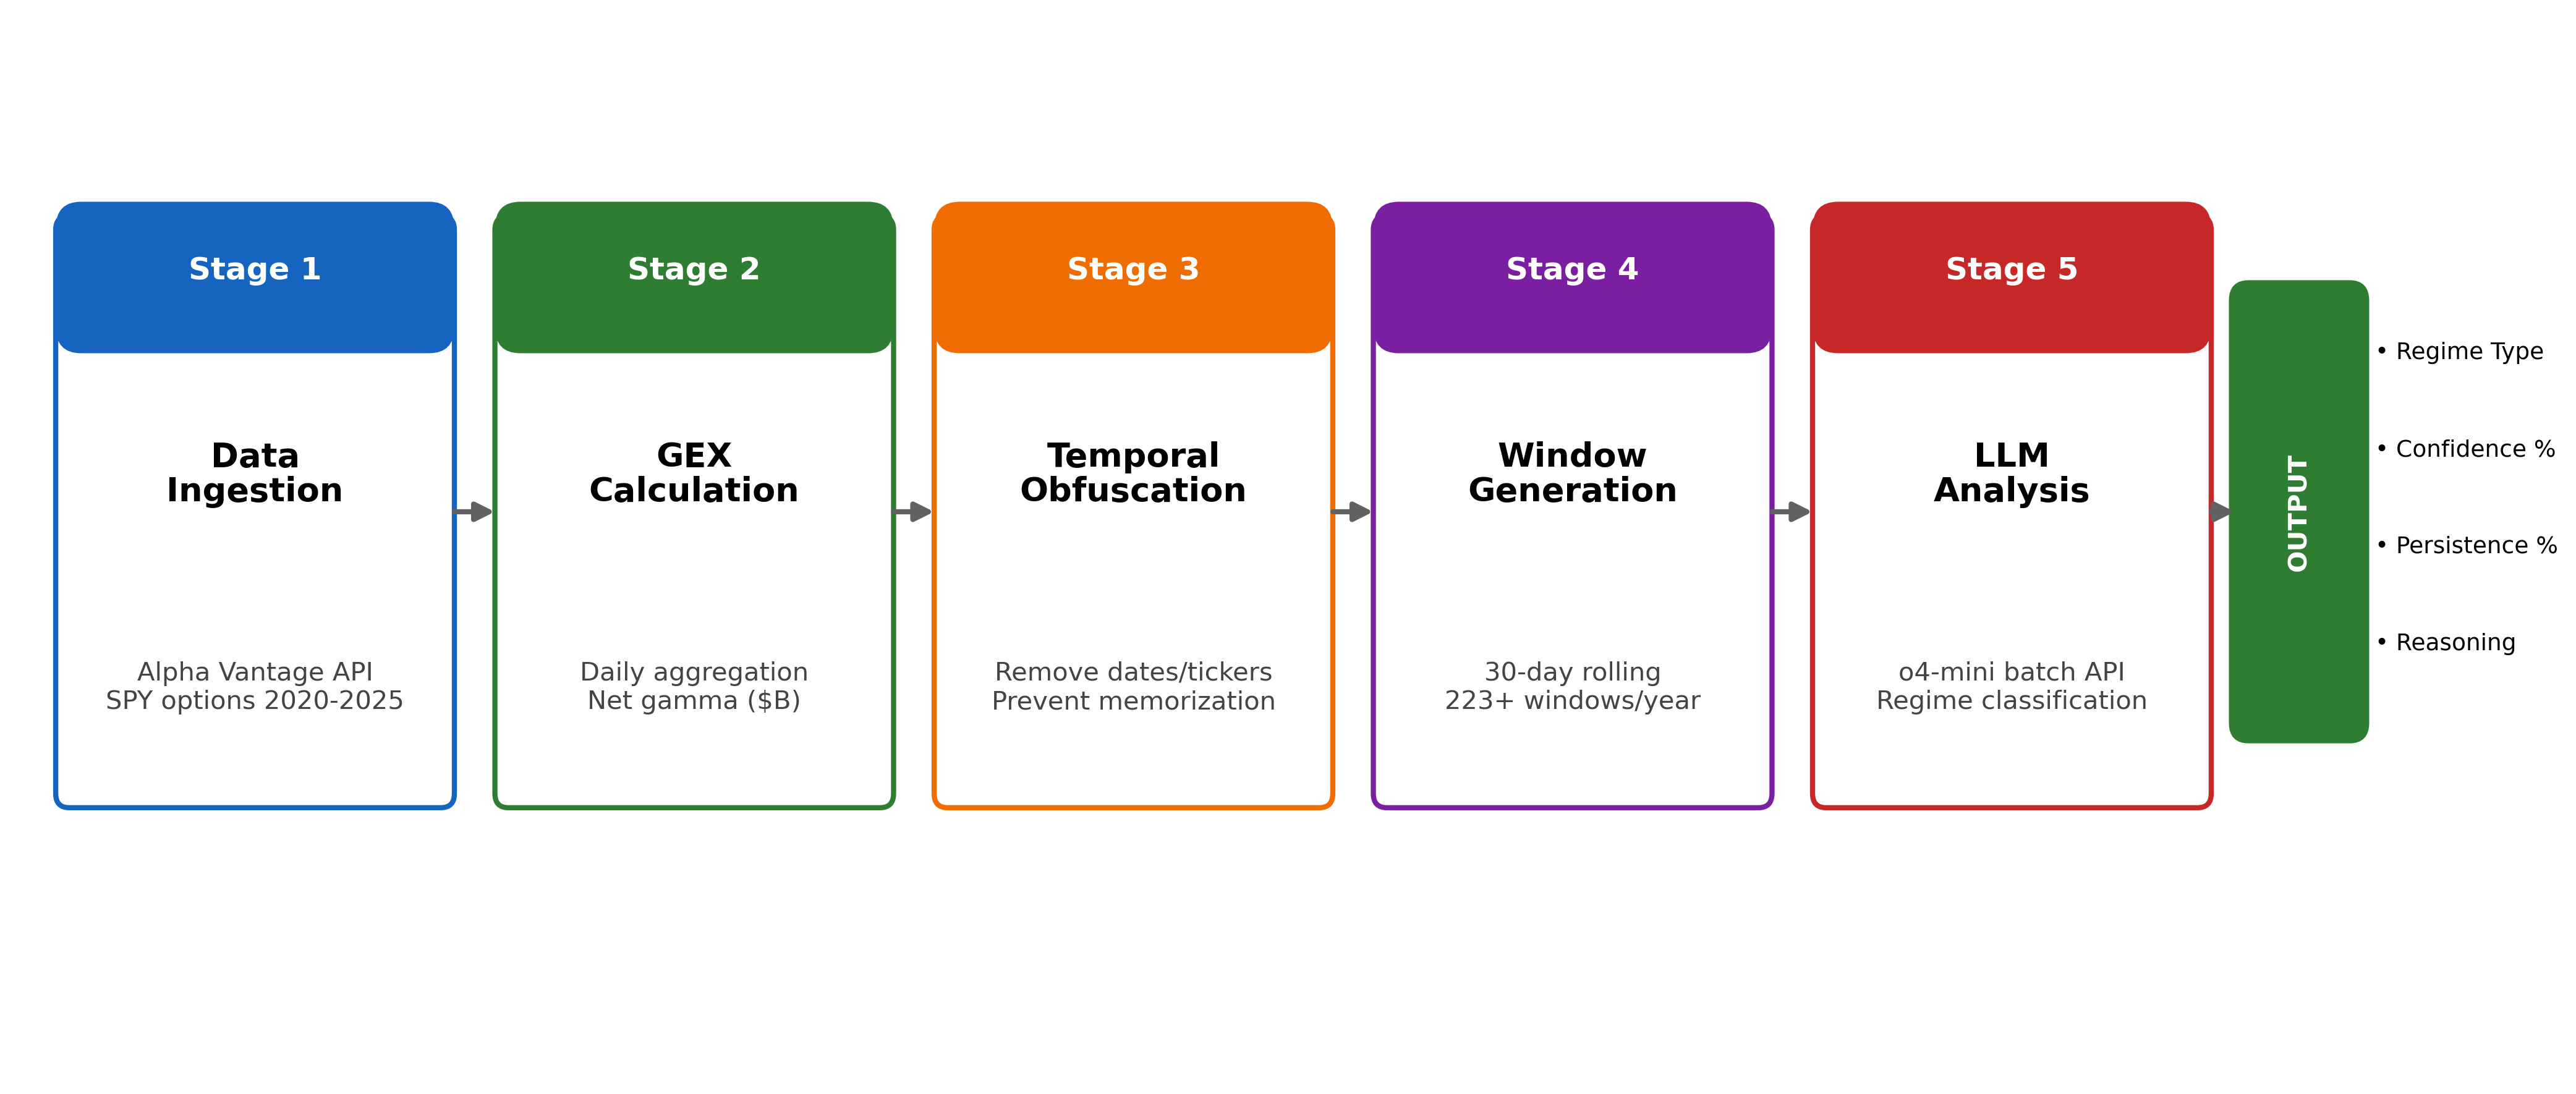
\includegraphics[width=\textwidth]{../figures/output/fig01_architecture.png}
\caption{LLM Regime Detection System Architecture. The pipeline processes trading days through five stages: data ingestion from Alpha Vantage API, GEX calculation with OI/Volume aggregation, temporal obfuscation to prevent memorization, 30-day window generation, and LLM analysis using OpenAI o4-mini via Batch API.}
\label{fig:architecture}
\end{figure*}

\subsection{30-Day Regime Detection Framework}

Building on the single-day obfuscation methodology from our prior work~\cite{regan2025obfuscation}, we extend the framework to detect \textit{persistent market regimes} rather than daily hedging patterns. A regime is defined as a 30-day window exhibiting sustained dealer gamma positioning that creates predictable market dynamics.

\subsubsection{Regime Classification Criteria}

We classify 30-day windows into four categories based on three structural metrics:

\textbf{Persistence}: Fraction of days sharing the dominant GEX sign
\begin{equation}
P = \frac{\text{days with dominant sign}}{30} \geq 0.70
\end{equation}

\textbf{Magnitude}: Average absolute gamma exposure
\begin{equation}
M = \frac{1}{30}\sum_{i=1}^{30} |\text{GEX}_i| \geq \$5\text{B}
\end{equation}

\textbf{Stability}: Maximum number of sign flips across 30 days
\begin{equation}
S = \text{count}(\text{sign}(\text{GEX}_{i+1}) \neq \text{sign}(\text{GEX}_i)) \leq 5
\end{equation}

\textbf{Regime Types}:
\begin{itemize}
\item \textbf{Persistent Positive}: $P \geq 0.70$, $M \geq \$5$B, $S \leq 5$, dominant sign positive
\item \textbf{Persistent Negative}: $P \geq 0.70$, $M \geq \$5$B, $S \leq 5$, dominant sign negative
\item \textbf{Transitional}: Fails persistence criterion ($P < 0.70$) or stability criterion ($S > 5$)
\item \textbf{Low Conviction}: Meets persistence/stability but $M < \$5$B
\end{itemize}

These thresholds were derived from principled criteria to isolate structurally significant positioning from background noise. The \$5B magnitude threshold reflects dealer risk management practices from financial microstructure literature, while 70\% persistence ensures detected regimes exhibit directional bias significantly exceeding random binomial variation ($\approx 2.2\sigma$ above chance).

\begin{figure}[!htbp]
\centering
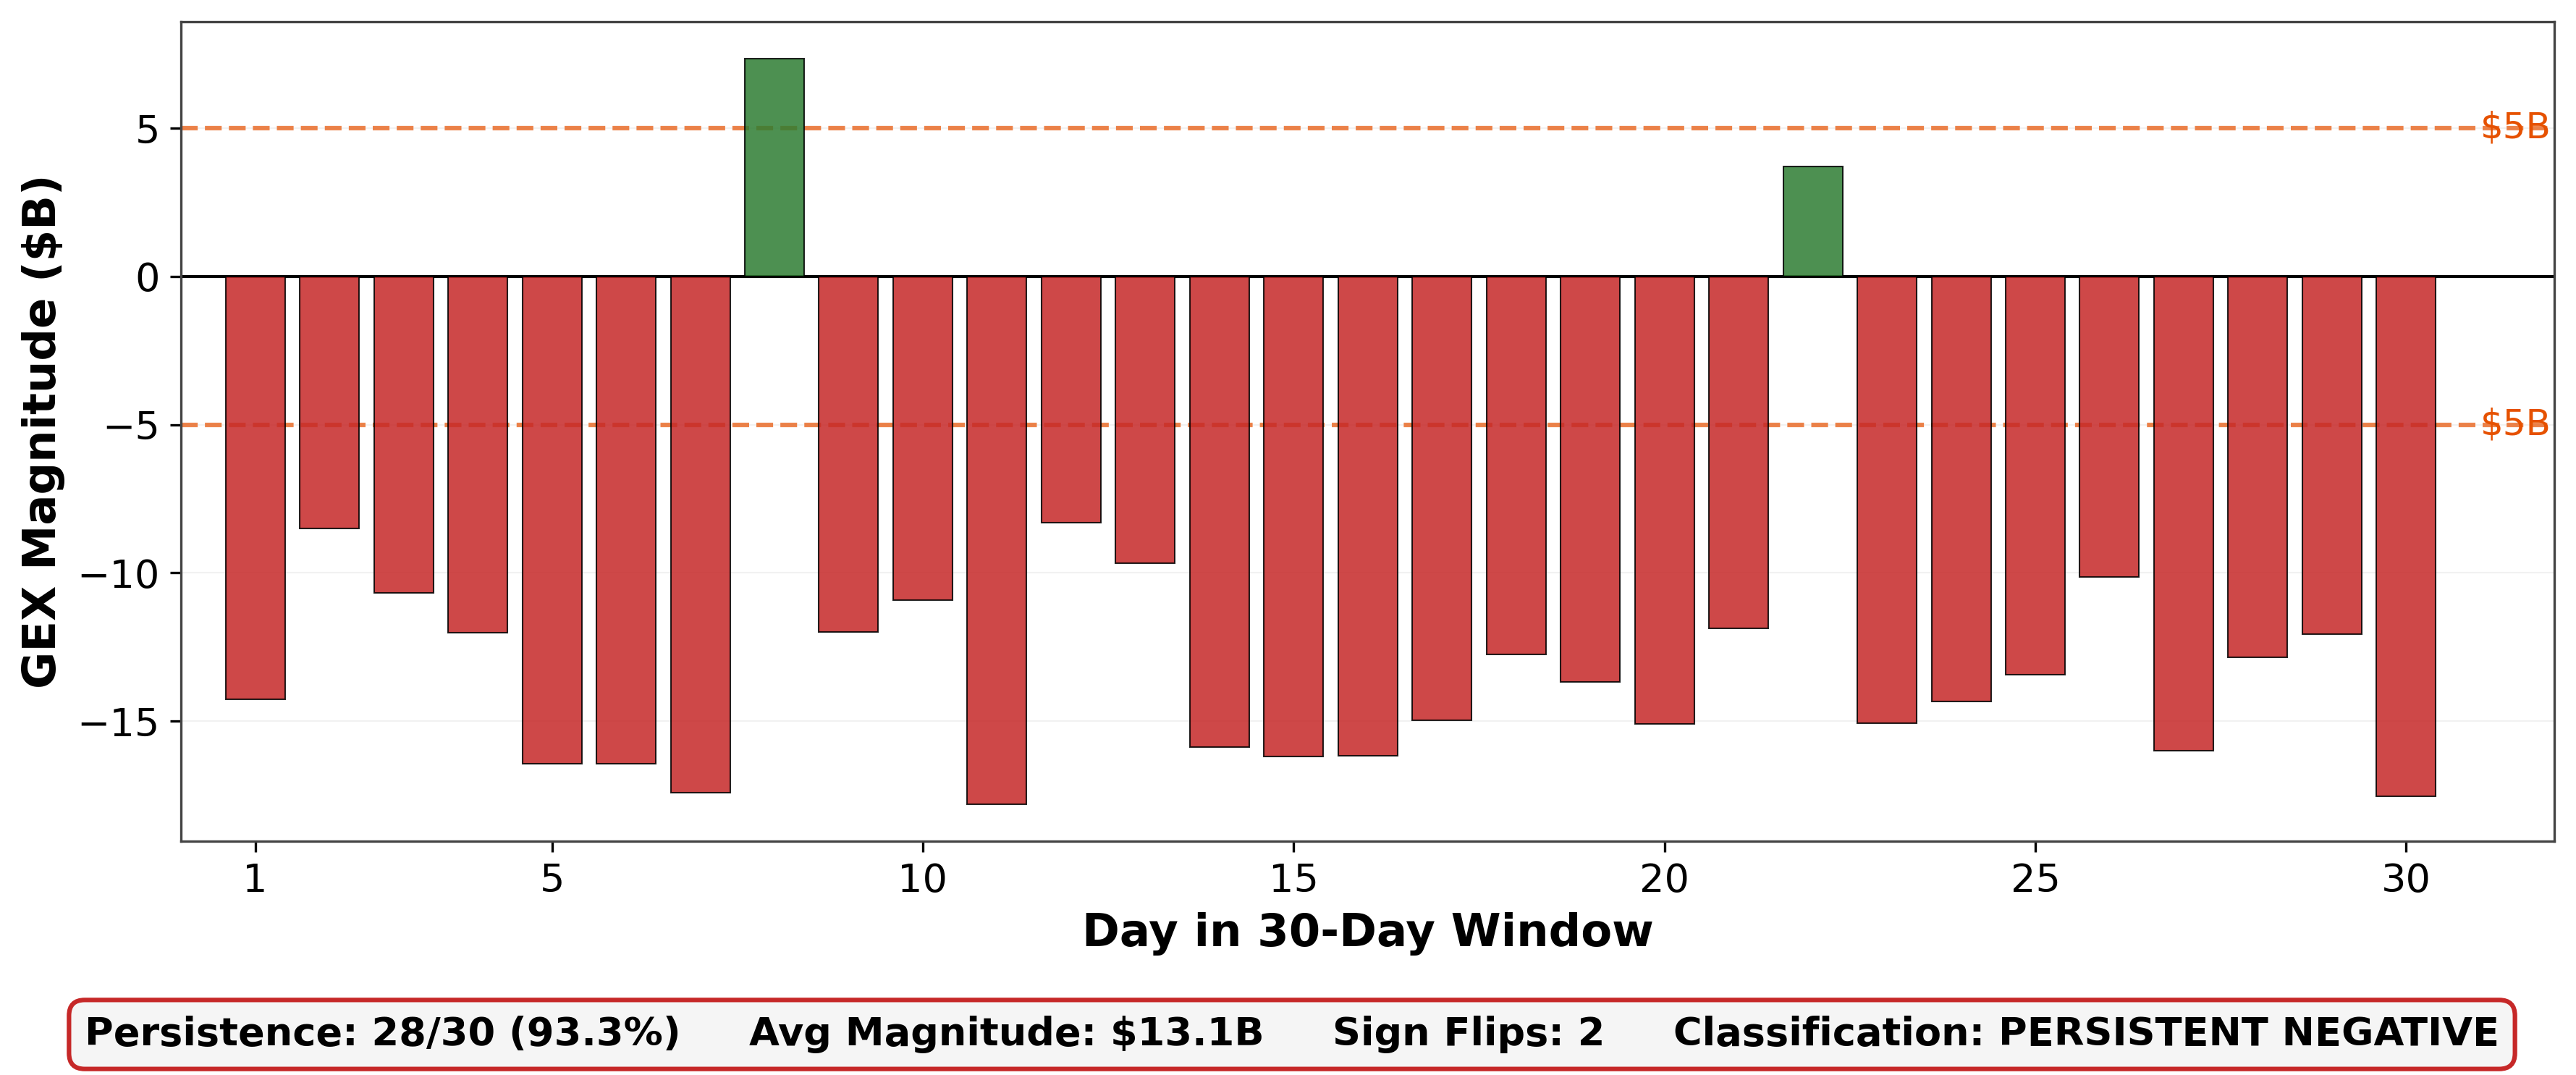
\includegraphics[width=\columnwidth]{../figures/output/fig02_regime_window.png}
\caption{30-Day Persistent Negative Regime Example. Daily GEX values showing 28/30 days negative (93.3\% persistence), average magnitude \$14.1B, and only 2 sign flips. All three detection criteria pass, triggering regime classification.}
\label{fig:regime_window}
\end{figure}

\subsection{GEX Calculation Methodology}

Following standard market microstructure practice~\cite{anderegg2022impact,spotgamma2021}, we calculate dealer gamma exposure from end-of-day open interest:

\begin{equation}
\text{GEX} = \sum_i \pm \text{OI}_i \times \Gamma_i \times S^2 \times 0.01 \times 100
\end{equation}

where $\Gamma_i$ is the Black-Scholes gamma at strike $i$, $\text{OI}_i$ is open interest, the factor of 100 converts contracts to shares, and $S^2$ scales gamma to dollar exposure. Call gamma enters positively, while put gamma enters negatively.

\subsubsection{Methodology Limitations}

This \textit{open interest-based} approach (GEX\_OI) measures dealer inventory positioning rather than intraday flow. While volume-based GEX (GEX\_VOL) may better capture 0DTE hedging dynamics, our regime detection framework is robust to measurement method because:

\begin{enumerate}
\item \textbf{Temporal aggregation}: 30-day windows smooth out daily measurement noise
\item \textbf{Negative controls validated}: Framework rejects randomized and transitional data (Phase 2)
\item \textbf{0DTE comparison}: Phase 4 tests whether OI-based regimes differ pre/post-0DTE era (2020 vs 2024)
\end{enumerate}

Critically, dealers must maintain delta neutrality regardless of whether gamma is measured from open interest or order flow—the underlying hedging mechanism remains constant~\cite{dim2025zero,ni2005stock}. Our LLM detection approach validates structural signals through forward return materialization rather than relying solely on GEX formula precision.

\subsection{Obfuscation Testing}

To prevent temporal memorization, we apply the same obfuscation protocol from our prior work~\cite{regan2025obfuscation}. Figure~\ref{fig:obfuscation} contrasts the raw data (left panel, with calendar dates, ticker symbols, and temporal context) against the obfuscated input (right panel), demonstrating how the transformation strips identifiable features while preserving structural information:

\begin{itemize}
\item Calendar dates → Relative labels ("Day T-29" through "Day T+0")
\item Ticker symbols → Generic identifier ("INDEX\_1")
\item No event labels, news references, or regime indicators
\item Present only: GEX magnitudes, spot prices, days to expiration
\end{itemize}

The LLM receives 30 consecutive GEX values with no contextual information, forcing purely structural reasoning about dealer constraints.

\begin{figure}[!htbp]
\centering
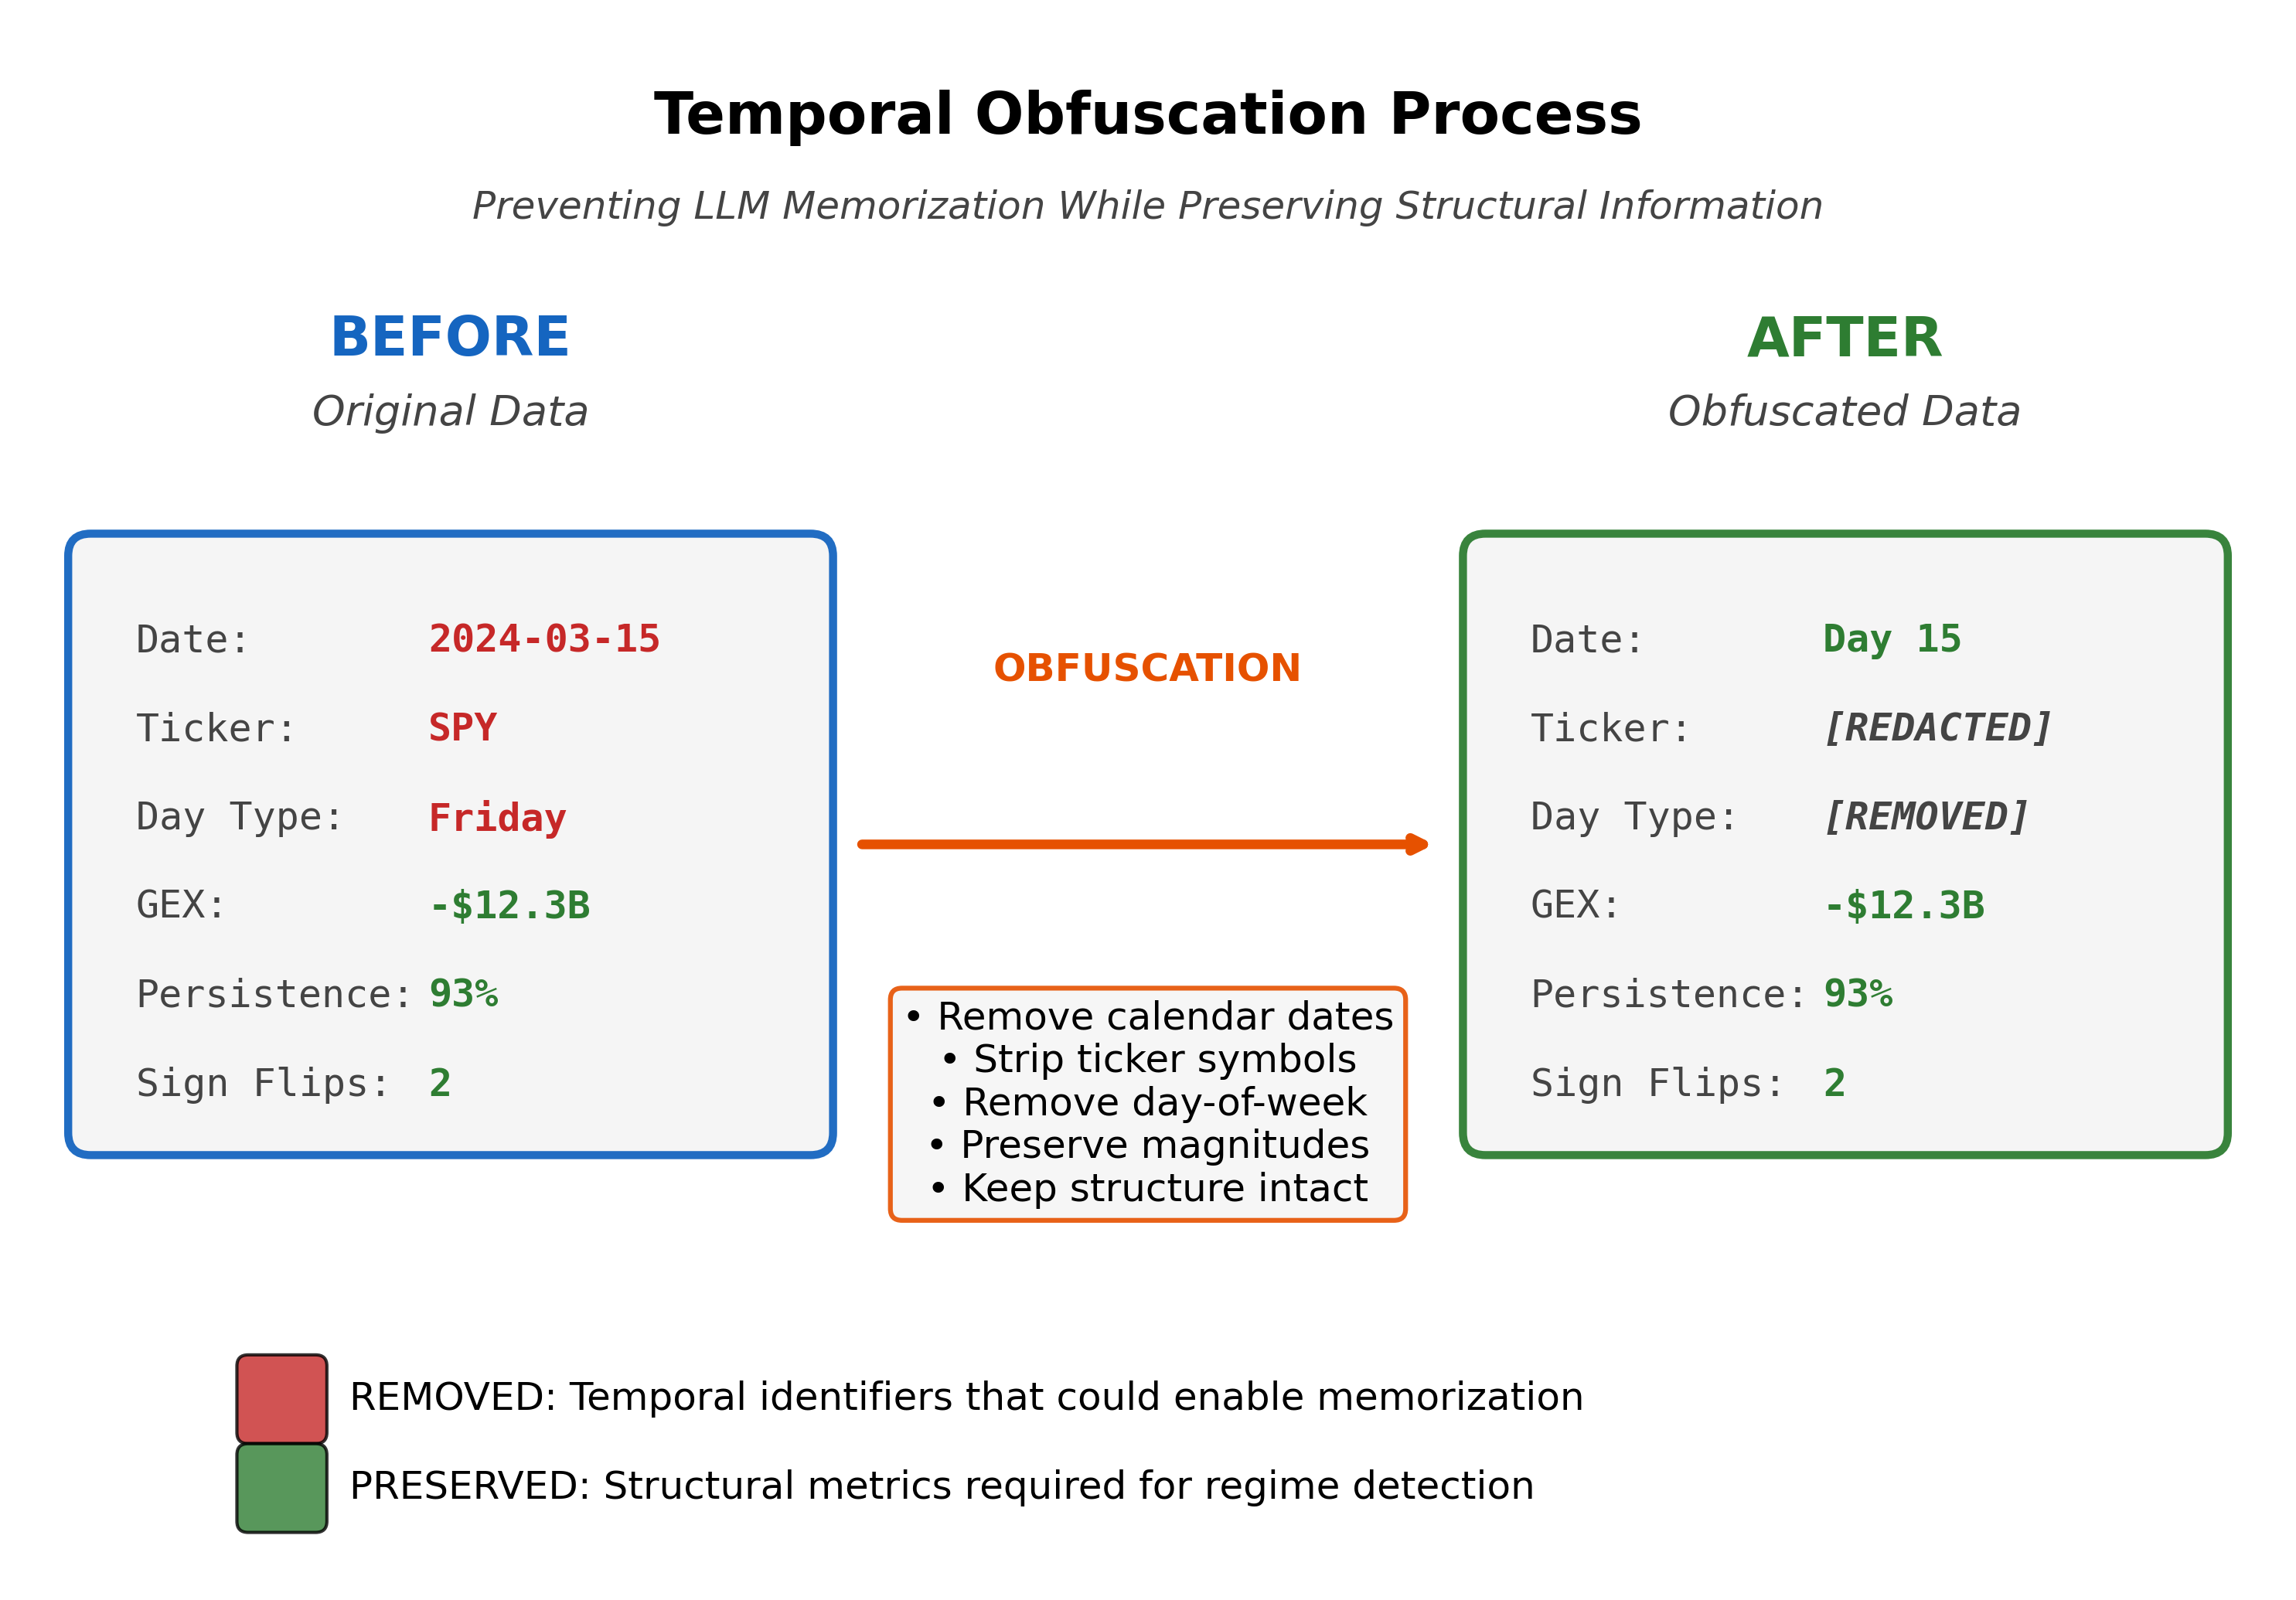
\includegraphics[width=0.48\textwidth]{../figures/output/fig03_obfuscation.png}
\caption{Temporal Obfuscation Process. Calendar dates, ticker symbols, and temporal context are removed while preserving GEX magnitude and structural relationships.}
\label{fig:obfuscation}
\end{figure}

\subsection{Multi-Phase Validation Strategy}

To ensure methodological rigor and avoid false positives, we implemented a comprehensive validation protocol spanning two critical years (2020 pre-0DTE, 2024 post-0DTE):

\vspace{0.2cm}

\subsubsection{Phase 1: Q1 2024 Baseline (52 windows)}

Establish baseline detection rate on Q1 2024 data (January 2 - March 27, 2024). Success criteria: 30-50\% detection rate demonstrating framework selectivity, not universal pattern matching.

\vspace{0.2cm}

\subsubsection{Phase 2: Negative Controls (809 windows)}

Validate framework discrimination using three synthetic tests:

\vspace{0.1cm}

\noindent\textbf{Phase 2a - Shuffle Test} (404 windows): Randomize day order within real 30-day sequences to destroy temporal structure while preserving statistical properties. Expected: $<$20\% false positive rate.

\vspace{0.1cm}

\noindent\textbf{Phase 2b - Transitional Test} (202 windows): Filter for high-volatility periods with 7-10 sign flips. Expected: $<$10\% false positive rate (should reject as non-regimes).

\vspace{0.1cm}

\noindent\textbf{Phase 2c - Low-Magnitude Test} (203 windows): Scale persistent sequences by 75\% to fall below \$5B threshold. Expected: $<$10\% false positive rate (should reject as low conviction).

\vspace{0.2cm}

\subsubsection{Phase 3: Full 2024 Validation (223 windows)}

If Phase 1-2 pass, validate across full 2024 year (all 252 trading days). This tests whether Q1 results generalize across different market conditions including February-March volatility.

\vspace{0.2cm}

\subsubsection{Phase 4: 2020 Comparison (223 windows)}

Test pre-0DTE era (2020) to validate the hypothesis that 0DTE proliferation increased regime persistence. Expected: Lower detection rate in 2020 vs 2024, establishing baseline for normal market fragmentation.

\subsection{LLM Detection Pipeline}

For each 30-day window:

\begin{enumerate}
\item \textbf{Prepare obfuscated prompt}: 30-day GEX sequence with relative date labels
\item \textbf{LLM structural reasoning}: Model analyzes persistence, magnitude, stability
\item \textbf{Classification}: Regime type (persistent\_positive, persistent\_negative, transitional, low\_conviction)
\item \textbf{Confidence scoring}: 0-100 scale based on criteria satisfaction
\item \textbf{Mechanical verification}: Compare LLM metrics vs actual window statistics
\end{enumerate}

We use OpenAI's o4-mini reasoning model with temperature=1.0 to generate explicit step-by-step analysis of regime characteristics. The model was selected for its chain-of-thought reasoning capabilities, which enable transparent identification of structural constraints~\cite{openai2024reasoning}.

\subsection{Statistical Framework}

We assess framework performance through three primary metrics:

\vspace{0.3cm}

\noindent\textbf{Detection Rate}: Fraction of windows classified as persistent regimes.

\begin{equation}
\text{DR} = \frac{\text{persistent regimes detected}}{\text{total windows}}
\end{equation}

\vspace{0.2cm}

\noindent\textbf{Selectivity Metrics}: Discrimination between real and synthetic data measured through:

\begin{itemize}
\item Persistence gap: $P_{\text{detected}} - P_{\text{rejected}}$ (percentage points)
\item Magnitude gap: $M_{\text{detected}} - M_{\text{rejected}}$ (billions USD)
\item Confidence gap: $C_{\text{detected}} - C_{\text{rejected}}$ (0-100 scale)
\end{itemize}

\vspace{0.2cm}

\noindent\textbf{Market Structure Evolution}: Cross-period detection difference quantifies structural change.

\begin{equation}
\Delta_{\text{period}} = \text{DR}_{\text{year}_2} - \text{DR}_{\text{year}_1}
\end{equation}

A large positive $\Delta_{\text{period}}$ (e.g., $>$50 percentage points) indicates fundamental market structure shift. We test this between 2020 (pre-0DTE) and 2024 (post-0DTE) to quantify the market structure difference between eras.
